\documentclass[11pt]{article}
\usepackage{mathblatt}
% gesetzt von werkzeuge/setzer.py aus dem Lernweg (L1-A · L1-B · L1-C · L1-D · L1-E · L1-T) und den Bankzeilen; Muster T6B.
\input{praeambel}
\newcommand{\kennung}{QG4}
\newcommand{\grau}[1]{{\color{mbgrau}#1}}

\begin{document}
\pfheftstil
\fancyfoot[C]{\parbox[t]{\textwidth}{\mbfhbox\par\vspace{1.5mm}{\footnotesize\color{mbgrau}{\scriptsize \kennung}\hfill\thepage}}}
\pfheftkopf{Bruch als Anteil}{Klasse 7}
% L1-A: Anteil ablesen: Zähler und Nenner
\begin{pfaufg}{}{1.}{}
\gzwei{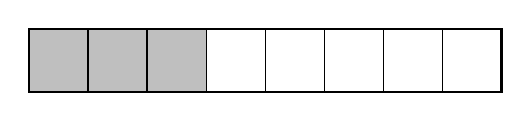
\begin{tikzpicture}[line cap=round]\fill[black!25] (0.000,0) rectangle (0.750,0.8);\draw[line width=0.4pt] (0.000,0) -- (0.000,0.8);\fill[black!25] (0.750,0) rectangle (1.500,0.8);\draw[line width=0.4pt] (0.750,0) -- (0.750,0.8);\fill[black!25] (1.500,0) rectangle (2.250,0.8);\draw[line width=0.4pt] (1.500,0) -- (1.500,0.8);\draw[line width=0.4pt] (2.250,0) -- (2.250,0.8);\draw[line width=0.4pt] (3.000,0) -- (3.000,0.8);\draw[line width=0.4pt] (3.750,0) -- (3.750,0.8);\draw[line width=0.4pt] (4.500,0) -- (4.500,0.8);\draw[line width=0.4pt] (5.250,0) -- (5.250,0.8);\draw[line width=0.9pt] (0,0) rectangle (6.0,0.8);\end{tikzpicture}}{\grau{a)\ Der Streifen ist in gleich große Teile geteilt. Welcher Anteil des Streifens ist grau?\par\smallskip Alle Teile zählen: 8 gleich große Teile. Das ist der Nenner.\par Graue Teile zählen: 3. Das ist der Zähler.\par Anteil: $\frac{3}{8}$ des Streifens ist grau.\par Probe: 3 graue und 5 weiße Teile sind zusammen 8 – gezählt wird das Ganze, nicht nur der Rest.}}
\par\medskip
\gzwei{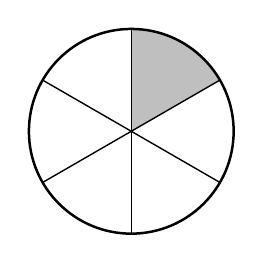
\begin{tikzpicture}[line cap=round]\fill[black!25] (0,0) -- (90:1.3) arc (90:30:1.3) -- cycle;\draw[line width=0.5pt] (0,0) -- (90:1.3);\draw[line width=0.5pt] (0,0) -- (30:1.3);\draw[line width=0.5pt] (0,0) -- (-30:1.3);\draw[line width=0.5pt] (0,0) -- (-90:1.3);\draw[line width=0.5pt] (0,0) -- (-150:1.3);\draw[line width=0.5pt] (0,0) -- (-210:1.3);\draw[line width=0.9pt] (0,0) circle (1.3);\end{tikzpicture}}{%
b)\ Der Kreis ist in gleich große Teile geteilt. Welcher Anteil des Kreises ist grau?\karo{3}}
\fusshilfe{\mbox{1:~b) $\frac{1}{6}$}}
\end{pfaufg}

% L1-A: Anteil ablesen: Zähler und Nenner
\begin{pfaufg}{}{2.}{}
\gzwei{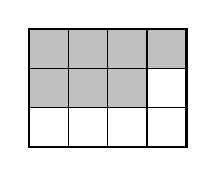
\begin{tikzpicture}[x=0.5cm,y=0.5cm,line cap=round]\fill[black!25] (0,2) rectangle (1,3);\fill[black!25] (1,2) rectangle (2,3);\fill[black!25] (2,2) rectangle (3,3);\fill[black!25] (3,2) rectangle (4,3);\fill[black!25] (0,1) rectangle (1,2);\fill[black!25] (1,1) rectangle (2,2);\fill[black!25] (2,1) rectangle (3,2);\draw[line width=0.4pt,step=1] (0,0) grid (4,3);\draw[line width=0.9pt] (0,0) rectangle (4,3);\end{tikzpicture}}{%
Die Figur besteht aus gleich großen Kästchen. Welcher Anteil der Figur ist grau?\karo{3}}
\fusshilfe{\mbox{2:~$\frac{7}{12}$}}
\end{pfaufg}

% L1-A: Anteil ablesen: Zähler und Nenner
\begin{pfaufg}{}{3.}{}
\gzwei{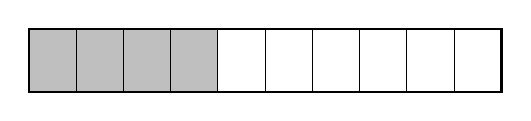
\begin{tikzpicture}[line cap=round]\fill[black!25] (0.000,0) rectangle (0.600,0.8);\draw[line width=0.4pt] (0.000,0) -- (0.000,0.8);\fill[black!25] (0.600,0) rectangle (1.200,0.8);\draw[line width=0.4pt] (0.600,0) -- (0.600,0.8);\fill[black!25] (1.200,0) rectangle (1.800,0.8);\draw[line width=0.4pt] (1.200,0) -- (1.200,0.8);\fill[black!25] (1.800,0) rectangle (2.400,0.8);\draw[line width=0.4pt] (1.800,0) -- (1.800,0.8);\draw[line width=0.4pt] (2.400,0) -- (2.400,0.8);\draw[line width=0.4pt] (3.000,0) -- (3.000,0.8);\draw[line width=0.4pt] (3.600,0) -- (3.600,0.8);\draw[line width=0.4pt] (4.200,0) -- (4.200,0.8);\draw[line width=0.4pt] (4.800,0) -- (4.800,0.8);\draw[line width=0.4pt] (5.400,0) -- (5.400,0.8);\draw[line width=0.9pt] (0,0) rectangle (6.0,0.8);\end{tikzpicture}}{%
Der Streifen ist in gleich große Teile geteilt. Welcher Anteil ist grau, welcher Anteil ist weiß?\karo{3}}
\fusshilfe{\mbox{3:~grau $\frac{4}{10}$, weiß $\frac{6}{10}$}}
\end{pfaufg}

% L1-A: Anteil ablesen: Zähler und Nenner
\begin{pfaufg}{}{4.}{}
In einer Klasse sind 24 Kinder, 11 davon sind Jungen. Welcher Anteil der Klasse sind Mädchen?\karo{3}
\fusshilfe{\mbox{4:~$\frac{13}{24}$}}
\end{pfaufg}

% L1-A: Anteil ablesen: Zähler und Nenner
\begin{pfaufg}{}{5.}{}
Beim Sportfest tragen in der Klasse 7a 12 von 24 Kindern ein rotes Shirt, in der Klasse 7b 10 von 20 Kindern. In welcher Klasse ist der Anteil der roten Shirts größer? Begründe.\karo{3}
\fusshilfe{\mbox{5:~In beiden Klassen gleich: je die Hälfte.}}
\end{pfaufg}

% L1-B: Anteil einzeichnen
\begin{pfaufg}{}{6.}{}
\gzwei{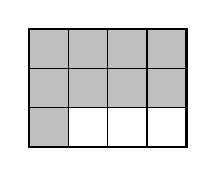
\begin{tikzpicture}[x=0.5cm,y=0.5cm,line cap=round]\fill[black!25] (0,2) rectangle (1,3);\fill[black!25] (1,2) rectangle (2,3);\fill[black!25] (2,2) rectangle (3,3);\fill[black!25] (3,2) rectangle (4,3);\fill[black!25] (0,1) rectangle (1,2);\fill[black!25] (1,1) rectangle (2,2);\fill[black!25] (2,1) rectangle (3,2);\fill[black!25] (3,1) rectangle (4,2);\fill[black!25] (0,0) rectangle (1,1);\draw[line width=0.4pt,step=1] (0,0) grid (4,3);\draw[line width=0.9pt] (0,0) rectangle (4,3);\end{tikzpicture}}{\grau{a)\ Die Figur besteht aus 12 gleich großen Kästchen. Färbe $\frac{3}{4}$ der Figur.\par\smallskip Nenner 4: Das Ganze wird in 4 gleiche Teile geteilt. $12 : 4 = 3$ – ein Viertel sind 3 Kästchen.\par Zähler 3: drei solche Teile. $3 \cdot 3 = 9$ Kästchen.\par 9 Kästchen färben (nicht 3 – der Zähler zählt Teile, nicht Kästchen).\par Probe: 3 Kästchen bleiben weiß, das ist das letzte Viertel.}}
\par\medskip
\gzwei{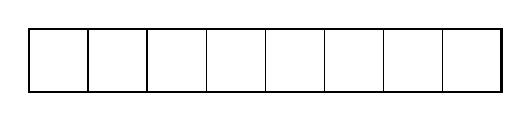
\begin{tikzpicture}[line cap=round]\draw[line width=0.4pt] (0.000,0) -- (0.000,0.8);\draw[line width=0.4pt] (0.750,0) -- (0.750,0.8);\draw[line width=0.4pt] (1.500,0) -- (1.500,0.8);\draw[line width=0.4pt] (2.250,0) -- (2.250,0.8);\draw[line width=0.4pt] (3.000,0) -- (3.000,0.8);\draw[line width=0.4pt] (3.750,0) -- (3.750,0.8);\draw[line width=0.4pt] (4.500,0) -- (4.500,0.8);\draw[line width=0.4pt] (5.250,0) -- (5.250,0.8);\draw[line width=0.9pt] (0,0) rectangle (6.0,0.8);\end{tikzpicture}}{%
b)\ Der Streifen ist in gleich große Teile geteilt. Färbe $\frac{5}{8}$ des Streifens.\karo{3}}
\fusshilfe{\mbox{6:~b) 5 Teile}}
\end{pfaufg}

% L1-B: Anteil einzeichnen
\begin{pfaufg}{}{7.}{}
\gzwei{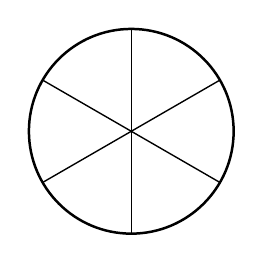
\begin{tikzpicture}[line cap=round]\draw[line width=0.5pt] (0,0) -- (90:1.3);\draw[line width=0.5pt] (0,0) -- (30:1.3);\draw[line width=0.5pt] (0,0) -- (-30:1.3);\draw[line width=0.5pt] (0,0) -- (-90:1.3);\draw[line width=0.5pt] (0,0) -- (-150:1.3);\draw[line width=0.5pt] (0,0) -- (-210:1.3);\draw[line width=0.9pt] (0,0) circle (1.3);\end{tikzpicture}}{%
Der Kreis ist in gleich große Teile geteilt. Färbe $\frac{2}{3}$ des Kreises.\karo{3}}
\fusshilfe{\mbox{7:~4 Teile}}
\end{pfaufg}

% L1-B: Anteil einzeichnen
\begin{pfaufg}{}{8.}{}
\gzwei{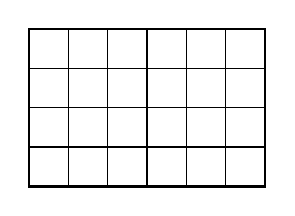
\begin{tikzpicture}[x=0.5cm,y=0.5cm,line cap=round]\draw[line width=0.4pt,step=1] (0,0) grid (6,4);\draw[line width=0.9pt] (0,0) rectangle (6,4);\end{tikzpicture}}{%
Die Figur besteht aus 24 gleich großen Kästchen. Schraffiere $\frac{5}{6}$ der Figur.\karo{3}}
\fusshilfe{\mbox{8:~20 Kästchen}}
\end{pfaufg}

% L1-B: Anteil einzeichnen
\begin{pfaufg}{}{9.}{}
\gzwei{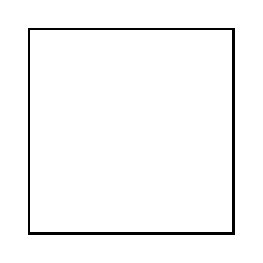
\begin{tikzpicture}\draw[line width=0.9pt] (0,0) rectangle (2.6,2.6);\end{tikzpicture}}{%
Die Figur zeigt ein leeres Quadrat. Kennzeichne ein Viertel seiner Fläche. Teile dazu das Quadrat zuerst in gleich große Teile.\karo{3}}
\fusshilfe{\mbox{9:~1 von 4 gleichen Teilen}}
\end{pfaufg}

% L1-B: Anteil einzeichnen
\begin{pfaufg}{}{10.}{}
Ein Beet hat 20 gleich große Felder. Auf $\frac{3}{5}$ der Felder sollen Tomaten wachsen, auf $\frac{1}{4}$ Salat. Reicht das Beet für beides? Wie viele Felder bleiben frei?\karo{3}
\fusshilfe{\mbox{10:~Ja, es reicht; 3 Felder bleiben frei.}}
\end{pfaufg}

% L1-C: Ungleiche Teile: erst gleich groß machen
\begin{pfaufg}{}{11.}{}
\gzwei{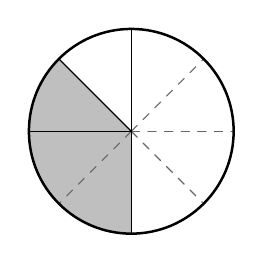
\begin{tikzpicture}[line cap=round]\fill[black!25] (0,0) -- (-90:1.3) arc (-90:-180:1.3) -- cycle;\fill[black!25] (0,0) -- (-180:1.3) arc (-180:-225:1.3) -- cycle;\draw[dashed,line width=0.4pt,black!60] (0,0) -- (0:1.3);\draw[dashed,line width=0.4pt,black!60] (0,0) -- (45:1.3);\draw[dashed,line width=0.4pt,black!60] (0,0) -- (180:1.3);\draw[dashed,line width=0.4pt,black!60] (0,0) -- (225:1.3);\draw[dashed,line width=0.4pt,black!60] (0,0) -- (270:1.3);\draw[dashed,line width=0.4pt,black!60] (0,0) -- (315:1.3);\draw[line width=0.5pt] (0,0) -- (90:1.3);\draw[line width=0.5pt] (0,0) -- (-90:1.3);\draw[line width=0.5pt] (0,0) -- (-180:1.3);\draw[line width=0.5pt] (0,0) -- (-225:1.3);\draw[line width=0.9pt] (0,0) circle (1.3);\end{tikzpicture}}{\grau{a)\ Der Kreis ist in verschieden große Teile geteilt. Welcher Anteil des Kreises ist grau?\par\smallskip Die Teile sind verschieden groß – so darf ich nicht zählen.\par Kleinstes Stück suchen: einer der zwei kleinen Sektoren links oben. Alles in solche Stücke teilen (gestrichelt): 8 Stücke. Nenner 8.\par Graue Stücke zählen: das große graue Stück sind 2 kleine, dazu 1 kleines: $2 + 1 = 3$. Zähler 3.\par Anteil $\frac{3}{8}$ – nicht $\frac{2}{4}$, denn 2 von 4 Teilen wäre nur richtig, wenn alle Teile gleich groß wären.}}
\par\medskip
\gzwei{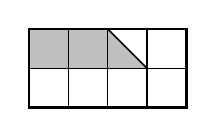
\begin{tikzpicture}[x=0.5cm,y=0.5cm,line cap=round]\fill[black!25] (0,1) rectangle (1,2);\fill[black!25] (1,1) rectangle (2,2);\fill[black!25] (2,1) -- (3,1) -- (2,2) -- cycle;\draw[line width=0.6pt] (3,1) -- (2,2);\draw[line width=0.4pt,step=1] (0,0) grid (4,2);\draw[line width=0.9pt] (0,0) rectangle (4,2);\end{tikzpicture}}{%
b)\ Das Rechteck besteht aus 8 Kästchen. Die schräge Linie teilt ein Kästchen in zwei Hälften. Welcher Anteil des Rechtecks ist grau?\karo{3}}
\fusshilfe{\mbox{11:~b) $\frac{5}{16}$}}
\end{pfaufg}

% L1-C: Ungleiche Teile: erst gleich groß machen
\begin{pfaufg}{}{12.}{}
\gzwei{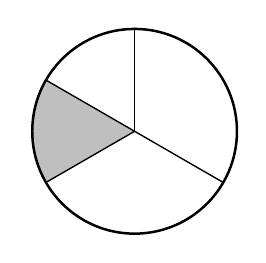
\begin{tikzpicture}[line cap=round]\fill[black!25] (0,0) -- (-150:1.3) arc (-150:-210:1.3) -- cycle;\draw[line width=0.5pt] (0,0) -- (90:1.3);\draw[line width=0.5pt] (0,0) -- (-30:1.3);\draw[line width=0.5pt] (0,0) -- (-150:1.3);\draw[line width=0.5pt] (0,0) -- (-210:1.3);\draw[line width=0.9pt] (0,0) circle (1.3);\end{tikzpicture}}{%
Der Kreis ist in verschieden große Teile geteilt. Welcher Anteil des Kreises ist grau?\karo{3}}
\fusshilfe{\mbox{12:~$\frac{1}{6}$}}
\end{pfaufg}

% L1-C: Ungleiche Teile: erst gleich groß machen
\begin{pfaufg}{}{13.}{}
\gzwei{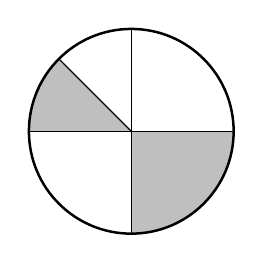
\begin{tikzpicture}[line cap=round]\fill[black!25] (0,0) -- (0:1.3) arc (0:-90:1.3) -- cycle;\fill[black!25] (0,0) -- (-180:1.3) arc (-180:-225:1.3) -- cycle;\draw[line width=0.5pt] (0,0) -- (90:1.3);\draw[line width=0.5pt] (0,0) -- (0:1.3);\draw[line width=0.5pt] (0,0) -- (-90:1.3);\draw[line width=0.5pt] (0,0) -- (-180:1.3);\draw[line width=0.5pt] (0,0) -- (-225:1.3);\draw[line width=0.9pt] (0,0) circle (1.3);\end{tikzpicture}}{%
Der Kreis ist in Sektoren geteilt. Die grauen Sektoren sind markiert. Kreuze an, welcher Anteil des Kreises markiert ist.\\\par\smallskip \gkreuz{$\frac{2}{5}$}\gkreuz{$\frac{3}{8}$}\par \gkreuz{$\frac{2}{8}$}\gkreuz{$\frac{3}{5}$}}
\fusshilfe{\mbox{13:~$\frac{3}{8}$}}
\end{pfaufg}

% L1-C: Ungleiche Teile: erst gleich groß machen
\begin{pfaufg}{}{14.}{}
\gzwei{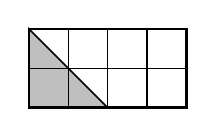
\begin{tikzpicture}[x=0.5cm,y=0.5cm,line cap=round]\fill[black!25] (0,0) -- (2,0) -- (0,2) -- cycle;\draw[line width=0.6pt] (0,0) -- (2,0) -- (0,2) -- cycle;\draw[line width=0.4pt,step=1] (0,0) grid (4,2);\draw[line width=0.9pt] (0,0) rectangle (4,2);\end{tikzpicture}}{%
Das Rechteck besteht aus 8 gleich großen Kästchen. Welcher Anteil des Rechtecks ist grau?\karo{3}}
\fusshilfe{\mbox{14:~$\frac{2}{8}$ $= \frac{1}{4}$}}
\end{pfaufg}

% L1-C: Ungleiche Teile: erst gleich groß machen
\begin{pfaufg}{}{15.}{}
Eine Pizza wird in 6 gleich große Stücke geschnitten. Ben schneidet ein Stück noch einmal in der Mitte durch. Er isst ein ganzes Stück und ein halbes. Welchen Anteil der Pizza hat Ben gegessen? Ist das mehr als ein Viertel, weniger oder genau ein Viertel?\karo{3}
\fusshilfe{\mbox{15:~$\frac{3}{12}$ $= \frac{1}{4}$, genau ein Viertel}}
\end{pfaufg}

% L1-D: Bruchteil einer Zahl oder Größe berechnen
\begin{pfaufg}{}{16.}{}
\grau{a)\ Berechne $\frac{3}{4}$ von $2{,}8$\,kg.\par\smallskip Durch den Nenner teilen: $2{,}8 : 4 = 0{,}7$ – das ist ein Viertel.\par Mal Zähler: $0{,}7 \cdot 3 = 2{,}1$ – drei Viertel.\par Antwort mit Einheit: $\frac{3}{4}$ von $2{,}8$\,kg sind $2{,}1$\,kg.\par Probe: Das Ergebnis ist kleiner als das Ganze, aber mehr als die Hälfte ($1{,}4$\,kg) – passt zu $\frac{3}{4}$.}
\par\medskip
b)\ Eine Schulstunde dauert 40 Minuten. $\frac{3}{8}$ der Stunde ist Gruppenarbeit. Wie viele Minuten sind das?\karo{3}
\fusshilfe{\mbox{16:~b) 15\,min}}
\end{pfaufg}

% L1-D: Bruchteil einer Zahl oder Größe berechnen
\begin{pfaufg}{}{17.}{}
Berechne $\frac{5}{6}$ von $1{,}8$\,l. Gib das Ergebnis in Liter an.\karo{3}
\fusshilfe{\mbox{17:~$1{,}5$\,l}}
\end{pfaufg}

% L1-D: Bruchteil einer Zahl oder Größe berechnen
\begin{pfaufg}{}{18.}{}
Ein Tank fasst 80\,l. Er ist zu $\frac{3}{5}$ gefüllt. Wie viele Liter fehlen bis zur vollen Füllung?\karo{3}
\fusshilfe{\mbox{18:~32\,l}}
\end{pfaufg}

% L1-D: Bruchteil einer Zahl oder Größe berechnen
\begin{pfaufg}{}{19.}{}
Ein Wanderweg ist $2{,}5$\,km lang. Nach $\frac{7}{10}$ des Weges kommt eine Bank. Wie viele Meter sind das?\karo{3}
\fusshilfe{\mbox{19:~1\,750\,m}}
\end{pfaufg}

% L1-D: Bruchteil einer Zahl oder Größe berechnen
\begin{pfaufg}{}{20.}{}
Eine Flasche fasst $0{,}75$\,l Saft. Lara trinkt zwei Drittel davon. Bleibt für ihren Bruder noch ein Viertelliter übrig? Begründe mit einer Rechnung.\karo{3}
\fusshilfe{\mbox{20:~Ja: Rest $0{,}25$\,l, genau ein Viertelliter.}}
\end{pfaufg}

% L1-E: Anteil in Prozent
\begin{pfaufg}{}{21.}{}
\gzwei{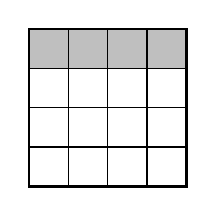
\begin{tikzpicture}[x=0.5cm,y=0.5cm,line cap=round]\fill[black!25] (0,3) rectangle (1,4);\fill[black!25] (1,3) rectangle (2,4);\fill[black!25] (2,3) rectangle (3,4);\fill[black!25] (3,3) rectangle (4,4);\draw[line width=0.4pt,step=1] (0,0) grid (4,4);\draw[line width=0.9pt] (0,0) rectangle (4,4);\end{tikzpicture}}{\grau{a)\ Die Figur besteht aus 16 gleich großen Kästchen. Markiere $25\,\%$ der Fläche.\par\smallskip Prozent in einen Bruch übersetzen: $25\,\% = \frac{25}{100} = \frac{1}{4}$.\par Wie in B: $16 : 4 = 4$ Kästchen sind ein Viertel.\par 4 Kästchen markieren – nicht 25, so viele gibt es gar nicht.\par Probe: 4 von 16 ist ein Viertel, und ein Viertel von 100 ist 25.}}
\par\medskip
\gzwei{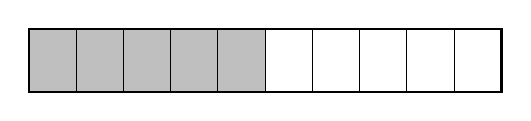
\begin{tikzpicture}[line cap=round]\fill[black!25] (0.000,0) rectangle (0.600,0.8);\draw[line width=0.4pt] (0.000,0) -- (0.000,0.8);\fill[black!25] (0.600,0) rectangle (1.200,0.8);\draw[line width=0.4pt] (0.600,0) -- (0.600,0.8);\fill[black!25] (1.200,0) rectangle (1.800,0.8);\draw[line width=0.4pt] (1.200,0) -- (1.200,0.8);\fill[black!25] (1.800,0) rectangle (2.400,0.8);\draw[line width=0.4pt] (1.800,0) -- (1.800,0.8);\fill[black!25] (2.400,0) rectangle (3.000,0.8);\draw[line width=0.4pt] (2.400,0) -- (2.400,0.8);\draw[line width=0.4pt] (3.000,0) -- (3.000,0.8);\draw[line width=0.4pt] (3.600,0) -- (3.600,0.8);\draw[line width=0.4pt] (4.200,0) -- (4.200,0.8);\draw[line width=0.4pt] (4.800,0) -- (4.800,0.8);\draw[line width=0.4pt] (5.400,0) -- (5.400,0.8);\draw[line width=0.9pt] (0,0) rectangle (6.0,0.8);\end{tikzpicture}}{%
b)\ Der Streifen ist in gleich große Teile geteilt. Welcher Anteil des Streifens ist grau? Gib den Anteil als Bruch und in Prozent an.\karo{3}}
\fusshilfe{\mbox{21:~b) $\frac{5}{10}$ $= \frac{1}{2} = 50\,\%$}}
\end{pfaufg}

% L1-E: Anteil in Prozent
\begin{pfaufg}{}{22.}{}
\gzwei{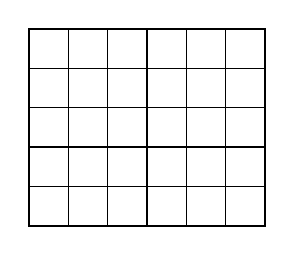
\begin{tikzpicture}[x=0.5cm,y=0.5cm,line cap=round]\draw[line width=0.4pt,step=1] (0,0) grid (6,5);\draw[line width=0.9pt] (0,0) rectangle (6,5);\end{tikzpicture}}{%
Die Figur besteht aus 30 gleich großen Kästchen. Markiere $20\,\%$ der Fläche.\karo{3}}
\fusshilfe{\mbox{22:~6 Kästchen}}
\end{pfaufg}

% L1-E: Anteil in Prozent
\begin{pfaufg}{}{23.}{}
\gzwei{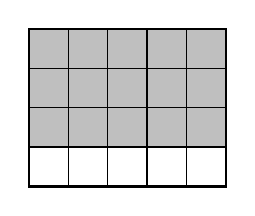
\begin{tikzpicture}[x=0.5cm,y=0.5cm,line cap=round]\fill[black!25] (0,3) rectangle (1,4);\fill[black!25] (1,3) rectangle (2,4);\fill[black!25] (2,3) rectangle (3,4);\fill[black!25] (3,3) rectangle (4,4);\fill[black!25] (4,3) rectangle (5,4);\fill[black!25] (0,2) rectangle (1,3);\fill[black!25] (1,2) rectangle (2,3);\fill[black!25] (2,2) rectangle (3,3);\fill[black!25] (3,2) rectangle (4,3);\fill[black!25] (4,2) rectangle (5,3);\fill[black!25] (0,1) rectangle (1,2);\fill[black!25] (1,1) rectangle (2,2);\fill[black!25] (2,1) rectangle (3,2);\fill[black!25] (3,1) rectangle (4,2);\fill[black!25] (4,1) rectangle (5,2);\draw[line width=0.4pt,step=1] (0,0) grid (5,4);\draw[line width=0.9pt] (0,0) rectangle (5,4);\end{tikzpicture}}{%
Die Figur besteht aus gleich großen Kästchen. Welcher Anteil der Figur ist grau? Gib den Anteil als Bruch und in Prozent an.\karo{3}}
\fusshilfe{\mbox{23:~$\frac{15}{20}$ $= \frac{3}{4} = 75\,\%$}}
\end{pfaufg}

% L1-E: Anteil in Prozent
\begin{pfaufg}{}{24.}{}
\gzwei{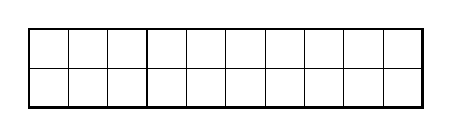
\begin{tikzpicture}[x=0.5cm,y=0.5cm,line cap=round]\draw[line width=0.4pt,step=1] (0,0) grid (10,2);\draw[line width=0.9pt] (0,0) rectangle (10,2);\end{tikzpicture}}{%
Die Figur besteht aus 20 gleich großen Kästchen. Markiere $10\,\%$ der Fläche.\karo{3}}
\fusshilfe{\mbox{24:~2 Kästchen}}
\end{pfaufg}

% L1-E: Anteil in Prozent
\begin{pfaufg}{}{25.}{}
Ein Parkhaus hat 40 Plätze, 30 davon sind besetzt. Ab $80\,\%$ Belegung zeigt die Anzeige am Eingang „fast voll“. Zeigt sie das jetzt an? Begründe mit einer Rechnung.\karo{3}
\fusshilfe{\mbox{25:~Nein: $75\,\%$ belegt, unter $80\,\%$.}}
\end{pfaufg}

% L1-T: Probetest
\begin{pfaufg}{}{26.}{}
\gzwei{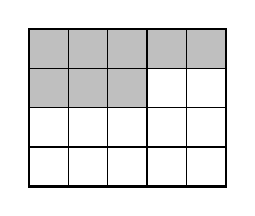
\begin{tikzpicture}[x=0.5cm,y=0.5cm,line cap=round]\fill[black!25] (0,3) rectangle (1,4);\fill[black!25] (1,3) rectangle (2,4);\fill[black!25] (2,3) rectangle (3,4);\fill[black!25] (3,3) rectangle (4,4);\fill[black!25] (4,3) rectangle (5,4);\fill[black!25] (0,2) rectangle (1,3);\fill[black!25] (1,2) rectangle (2,3);\fill[black!25] (2,2) rectangle (3,3);\draw[line width=0.4pt,step=1] (0,0) grid (5,4);\draw[line width=0.9pt] (0,0) rectangle (5,4);\end{tikzpicture}}{%
Die Figur besteht aus gleich großen Kästchen. Welcher Anteil der Figur ist grau? Gib den Anteil als Bruch und in Prozent an.\karo{3}}
\fusshilfe{\mbox{26:~$\frac{8}{20}$ $= \frac{2}{5} = 40\,\%$}}
\end{pfaufg}

% L1-T: Probetest
\begin{pfaufg}{}{27.}{}
\gzwei{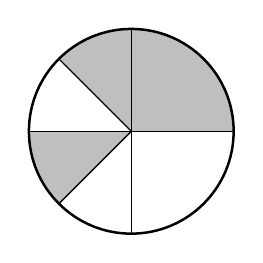
\begin{tikzpicture}[line cap=round]\fill[black!25] (0,0) -- (90:1.3) arc (90:0:1.3) -- cycle;\fill[black!25] (0,0) -- (-135:1.3) arc (-135:-180:1.3) -- cycle;\fill[black!25] (0,0) -- (-225:1.3) arc (-225:-270:1.3) -- cycle;\draw[line width=0.5pt] (0,0) -- (90:1.3);\draw[line width=0.5pt] (0,0) -- (0:1.3);\draw[line width=0.5pt] (0,0) -- (-90:1.3);\draw[line width=0.5pt] (0,0) -- (-135:1.3);\draw[line width=0.5pt] (0,0) -- (-180:1.3);\draw[line width=0.5pt] (0,0) -- (-225:1.3);\draw[line width=0.9pt] (0,0) circle (1.3);\end{tikzpicture}}{%
Der Kreis ist in Sektoren geteilt. Die grauen Sektoren sind markiert. Kreuze an, welcher Anteil des Kreises markiert ist.\\\par\smallskip \gkreuz{$\frac{3}{6}$}\gkreuz{$\frac{4}{8}$}\par \gkreuz{$\frac{3}{8}$}\gkreuz{$\frac{5}{8}$}}
\fusshilfe{\mbox{27:~$\frac{4}{8}$}}
\end{pfaufg}

% L1-T: Probetest
\begin{pfaufg}{}{28.}{}
\gzwei{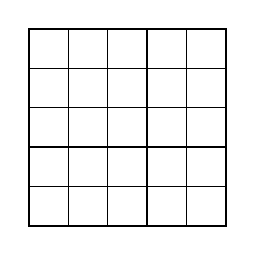
\begin{tikzpicture}[x=0.5cm,y=0.5cm,line cap=round]\draw[line width=0.4pt,step=1] (0,0) grid (5,5);\draw[line width=0.9pt] (0,0) rectangle (5,5);\end{tikzpicture}}{%
Die Figur besteht aus 25 gleich großen Kästchen. Schraffiere $\frac{3}{5}$ der Figur.\karo{3}}
\fusshilfe{\mbox{28:~15 Kästchen}}
\end{pfaufg}

% L1-T: Probetest
\begin{pfaufg}{}{29.}{}
Eine Regentonne fasst 900\,l. Sie ist zu $\frac{5}{6}$ gefüllt. Wie viele Liter passen noch hinein?\karo{3}
\fusshilfe{\mbox{29:~150\,l}}
\end{pfaufg}

% L1-T: Probetest
\begin{pfaufg}{}{30.}{}
Wie viel Gramm sind $\frac{5}{8}$ von $3{,}2$\,kg?\karo{3}
\fusshilfe{\mbox{30:~2\,000\,g}}
\end{pfaufg}

% L1-T: Probetest
\begin{pfaufg}{}{31.}{}
Eine Regentonne fasst 300\,l und ist zu $\frac{4}{5}$ gefüllt. In der Nacht laufen 50\,l Regenwasser hinein. Läuft die Tonne über? Begründe mit einer Rechnung.\karo{3}
\fusshilfe{\mbox{31:~Nein: 290\,l, es bleiben 10\,l Platz.}}
\end{pfaufg}

\par\vfill\noindent{\footnotesize Vorher: Teilen und Vervielfachen im Kopf\quad\textbullet\quad Weiter: Kürzen und Erweitern\par}
\end{document}
